\documentclass[conference]{IEEEtran}

\usepackage[utf8]{inputenc}
\usepackage{graphicx}
\usepackage{amsmath}
\usepackage{booktabs}
\usepackage{hyperref}
\usepackage{cite}

\title{
A Cyber Physical Inspection Assistant for Semi Automated Dimensional Quality Control in Smart Manufacturing
}

\author{
\IEEEauthorblockN{Your Name}
\IEEEauthorblockA{
Your Institution \\
Email: your.email@domain.com
}
}

\begin{document}

\maketitle

\begin{abstract}
Most assembly line dimensional inspections remain manual, creating bottlenecks as industries transition to Industry 4.0 processes. Small and medium sized enterprises lack low cost solutions that digitize quality inspection without requiring expensive metrology hardware or full automation.

This paper introduces a PC based Inspection Assistant designed to support manual measurement tasks using affordable digital tools. It reads real time data from USB digital vernier calipers, guides the operator step by step with short videos, and stores the results through a backend API connected to a structured database. A custom method filters out regular typing and accurately captures only the measurement input based on timing.

The system improves traceability, enforces a consistent workflow, and helps avoid manual errors, all while remaining simple enough for use on the assembly line. Future work will focus on testing it in real manufacturing settings to measure its practical impact.
\end{abstract}

\section{Introduction}
Dimensional inspection is essential to validating manufacturing tolerances. However, most operators still rely on manual measurement recording using digital calipers, notebooks, or spreadsheets. This introduces inefficiencies and limits traceability, especially as industries aim to adopt smart manufacturing practices.

Existing research focuses on fully automated cyber physical inspection systems, robotic metrology, and AI based quality assessment. However, these technologies remain costly and complex for widespread deployment. Semi manual workflows, still prevalent, lack structured digital support, real time data capture, and standardized logging.

To bridge this gap, a Cyber Physical Inspection Assistant was developed to support human operators rather than replace them. The system maintains traditional measurement tools while adding digital workflow structure, live instrument data capture, and automated validations.

\section{Related Work}
Most research in smart manufacturing focuses on either fully automated inspection or traditional manual setups with minimal digital support. But there is also a growing interest in hybrid systems that combine operator judgment with structured digital workflows.

\subsection{Automated and Sensor Driven Inspection Systems}
Castillo et al. (2024) developed a cyber physical inspection system for additive manufacturing that removes the operator entirely. Wang et al. (2024) presented a Human Cyber Physical framework for embedded quality assessment. These solutions offer speed and precision but require complex infrastructure, often unaffordable to small and medium sized enterprises.

\subsection{Operator Focused Models}
Ruppert et al.'s (2023) Operator 4.0 concept introduces wearable augmentation to re integrate humans into production. However, these approaches often prioritize monitoring and ergonomics over dimensional inspection.

\subsection{Digital Capture Tools and Interfaces}
Jwo et al. (2021) used OCR in a mobile app for capturing gauge readings. Ingole et al. (2014) built custom hardware to stream caliper data to a PC. However, these lacked workflow enforcement and digital traceability.

\subsection{Positioning This Work}
This Inspection Assistant fills a gap between manual logs and full automation. It introduces guided digital workflows, real time measurement capture, and traceable data logging using accessible and affordable technology. Rather than overhaul the inspection process, it augments what already exists on the assembly line.
\section{System Design and Implementation}

The Inspection Assistant was created with the specific objective of supporting existing assembly line processes rather than creating new ones.  The solution adds the digital advantages of traceability, structure, and speed while maintaining the familiarity of the human inspection process.  This makes it inexpensive and simple to implement, particularly for small and medium-sized businesses.
\subsection{Architecture Overview}
At the core of the system are components that connect are readily available and work together seamlessly:
\begin{itemize}
\item USB digital vernier caliper (HID compatible)
\item Flutter-based desktop interface
\item Python FastAPI backend
\item PostgreSQL database for structured storage
\end{itemize}

Figure~\ref{fig:system_architecture} shows the overall system layout. Each component is modular, so the system can maintain and evolve over time without redoing.

\begin{figure}[htbp]
\centering
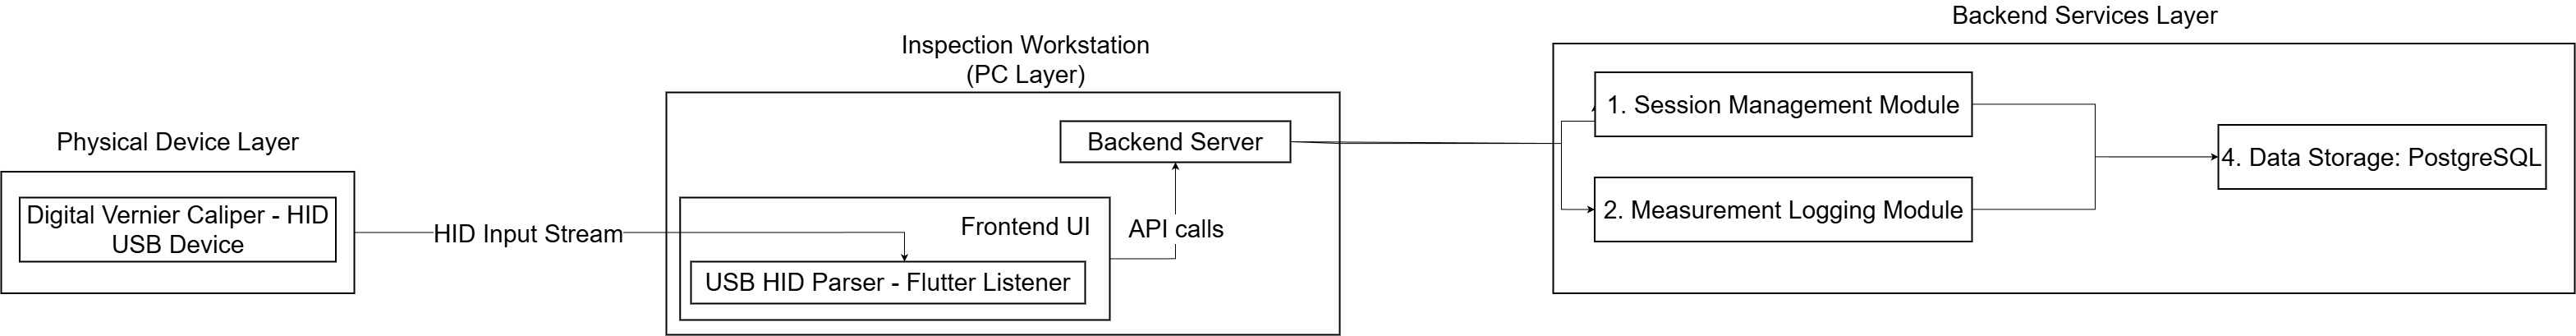
\includegraphics[width=0.9\linewidth]{System_architecture.jpg}
\caption{Overall System Architecture}
\label{fig:system_architecture}
\end{figure}

\subsection{Real Time Measurement Capture}
The digital caliper sends data over USB using the standard HID protocol. Instead of relying on complex drivers or vendor SDKs, the frontend listens for raw input through a hidden \texttt{TextField}. A custom timing filter detects high-density input bursts typical of instrument readings and filters out normal typing.

This approach:
\begin{itemize}
\item captures only the measurement values,
\item works cross platforms (e.g., Windows, Linux, Android),
\item and requires zero proprietary software.
\end{itemize}

The measurements are then parsed, validated, and sent to the backend.

\subsection{Modular Backend Architecture}
The backend handles validation, session tracking, template logic, and database storage. It’s split cleanly into:

\subsection{Backend and Data Handling Strategy}
The backend architecture is designed for modularity and clarity, allowing new inspection modules or workflows to be added without disrupting the existing system. It makes it possible to track, validate, and store operator sessions in a structured PostgreSQL database. Future growth to real-time dashboards, predictive analytics, and IIoT ecosystem integration is supported by this modular strategy.

All communication between the frontend and backend follows a RESTful pattern, abstracting the internal logic from the user-facing interface. This not only improves maintainability but also ensures compatibility with mobile and edge-based deployments in future work.
Figure~\ref{fig:backend_modules} illustrates the main backend modules and their interactions.
\begin{figure}[htbp]
\centering
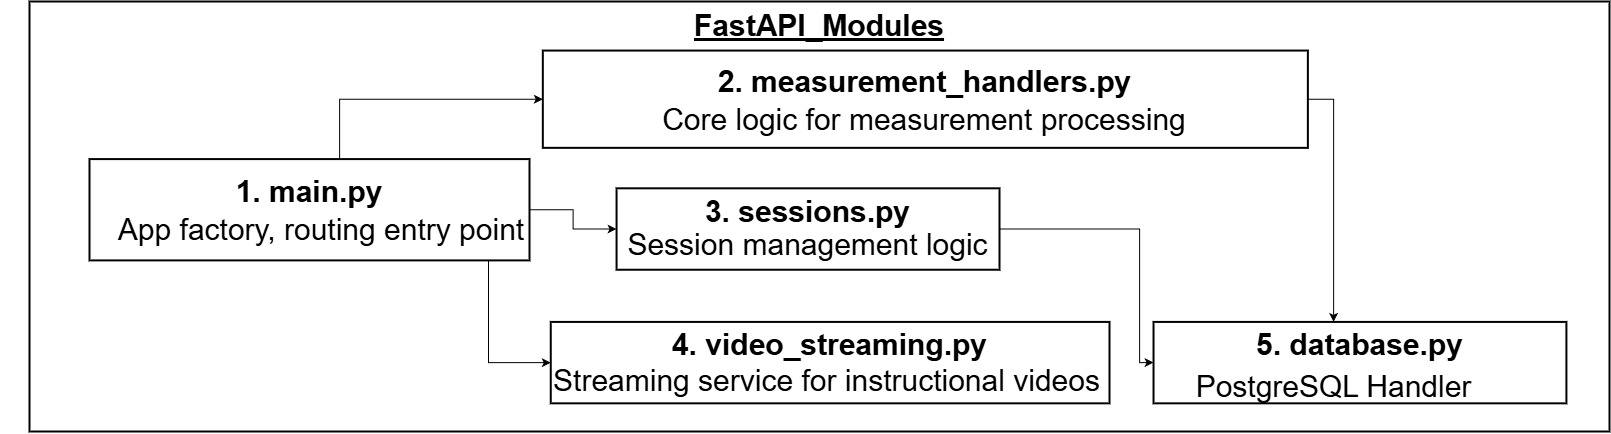
\includegraphics[width=0.9\linewidth]{backend_internal_diagram.jpg}
\caption{Backend Module Structure}
\label{fig:backend_modules}
\end{figure}

\subsection{Software Architecture Overview}
To give a complete picture, Figure~\ref{fig:software_architecture} shows how frontend, backend, and database components communicate during an inspection session. The flow is intentionally lightweight and quick to deploy.

\begin{figure}[htbp]
\centering
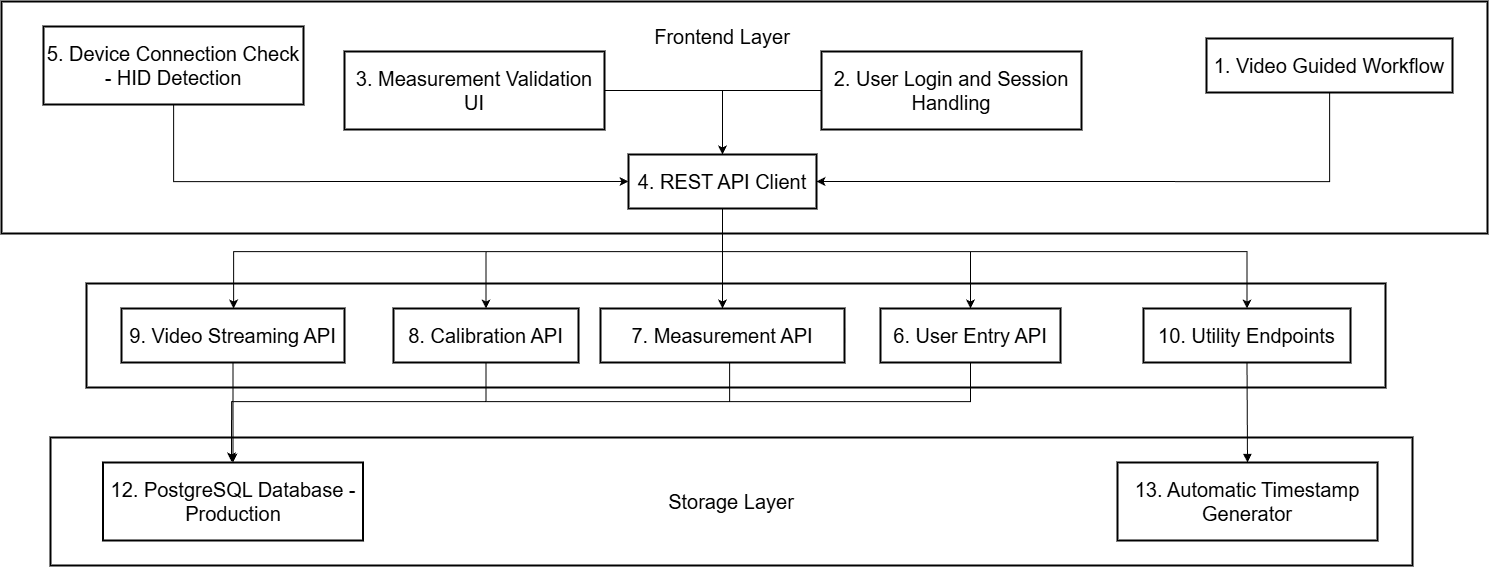
\includegraphics[width=0.9\linewidth]{Software_architecture.png}
\caption{Software Architecture Overview}
\label{fig:software_architecture}
\end{figure}

\subsection{Operator Workflow}
From the operator’s point of view, the system walks them through the inspection with clear steps:
\begin{enumerate}
\item Check that the device is connected
\item Log in
\item (Optional) calibrate the tool
\item Watch a short instructional clip
\item Record measurement
\item Submit results
\end{enumerate}

The workflow ensures each step is followed, reducing mistakes and keeping things consistent across shifts.

\begin{figure}[htbp]
\centering
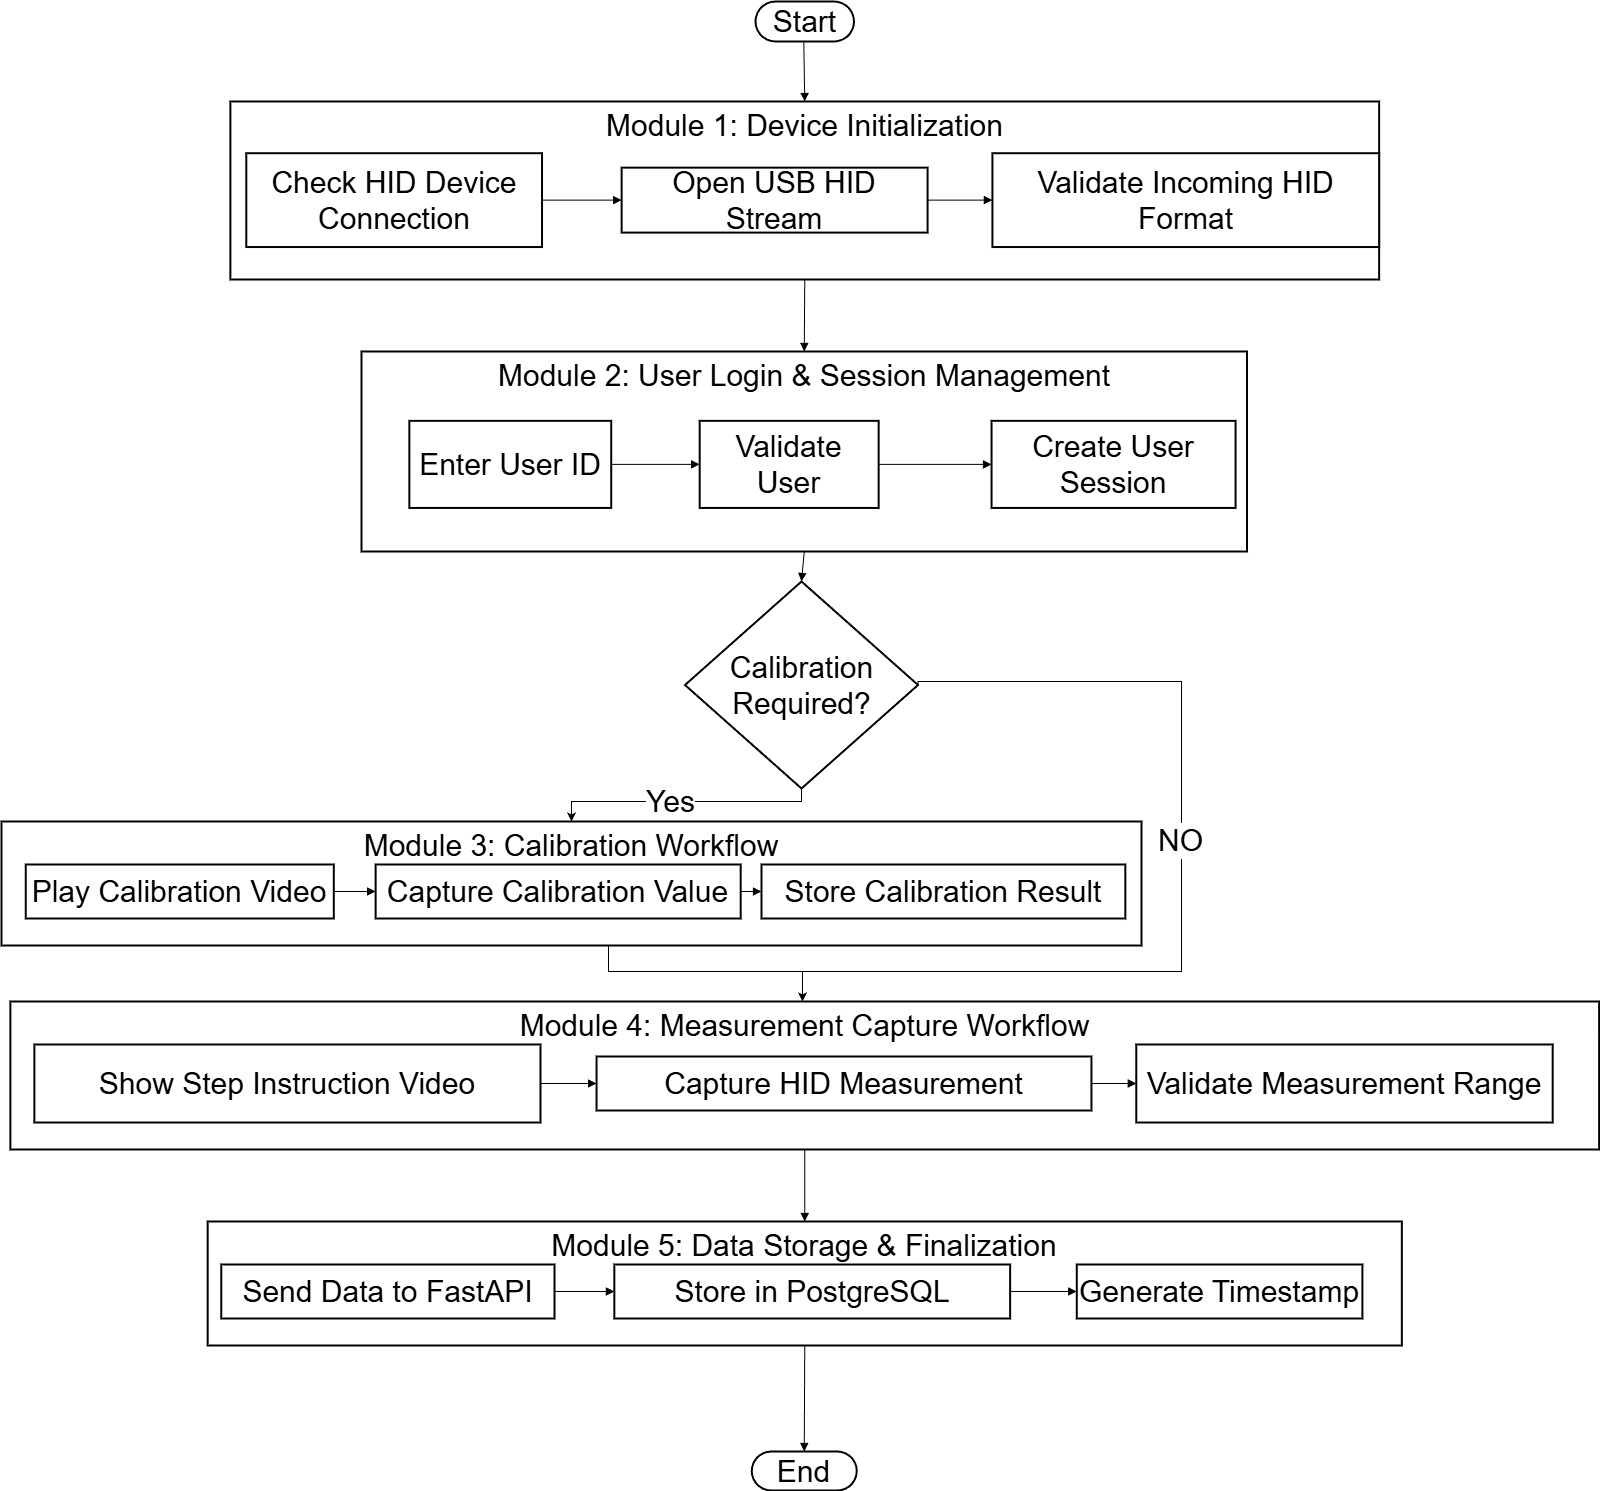
\includegraphics[width=0.9\linewidth]{WorkFlow_diagram.jpg}
\caption{Operator Workflow}
\label{fig:workflow}
\end{figure}


\section{Testing and Evaluation}
We evaluated the system in a lab setting that simulated actual assembly line conditions. Operators inspected shafts and housings using both traditional methods and the Inspection Assistant.

\subsection{Observations}
\begin{itemize}
\item \textbf{Errors}: Manual logging introduced 2 to 3 errors per 20 entries. These were eliminated with real time capture.
\item \textbf{Speed}: Digital guidance and automation reduced per part inspection time by 30 to 40 percent.
\item \textbf{Compliance}: All workflow steps were followed without skips when using the Assistant.
\item \textbf{Traceability}: Each record was timestamped and tagged to an operator session.
\end{itemize}

\subsection{Results Summary}
See Table \ref{tab:comparison} for a side by side comparison.

\begin{table}[htbp]
\centering
\caption{Manual vs Inspection Assistant Performance}
\begin{tabular}{lcc}
\toprule
\textbf{Metric} & \textbf{Manual} & \textbf{Assistant} \\
\midrule
Input Errors (per 20) & 2 to 3 & 0 \\
Time per Part (s) & 4.5 to 5.0 & 2.7 to 3.2 \\
Workflow Completion Rate & approx. 70\% & 100\% \\
Structured Digital Logs & No & Yes \\
\bottomrule
\end{tabular}
\label{tab:comparison}
\end{table}

\section{Discussion}
This system addresses a specific need in dimensional quality control: upgrading manual inspection stations with minimal disruption.  Without requiring expensive or complete automation, it enhances traceability, standardises processes, and prevents transcribing errors.

Because of its modular design, it can add new capabilities like IIoT connectivity or predictive analytics.
\section{Conclusion and Future Work}
The Inspection Assistant brings structured digital workflows and real time measurement capture to legacy manual stations. It supports human operators on the assembly line while aligning inspection tasks with Industry 4.0 goals.

Future work includes:
\begin{itemize}
\item Deployment on tablets and edge devices
\item Real time IIoT data streaming
\item Integration with predictive quality dashboards
\item Hybrid collaboration with robotic inspection systems
\end{itemize}

\bibliographystyle{IEEEtran}
\begin{thebibliography}{00}

\bibitem{markatos2023}
P. Markatos and A. Mousavi, ``Manufacturing quality assessment in the Industry 4.0 era,'' 2023. [Online]. Available: \url{https://bura.brunel.ac.uk/bitstream/2438/26299/1/FullText.pdf}

\bibitem{ruppert2023}
T. Ruppert \textit{et al.}, ``Operator 4.0 Retrofitting: A framework for worker-centered cyber-physical systems,'' \textit{Sensors}, 2023. [Online]. Available: \url{https://www.mdpi.com/1424-8220/23/14/6350}

\bibitem{wang2024}
L. Wang \textit{et al.}, ``Smart In Process Inspection using Cyber-Physical Systems,'' \textit{Machines}, 2024. [Online]. Available: \url{https://www.mdpi.com/2075-1702/12/1/4}

\bibitem{jwo2021}
D. Jwo \textit{et al.}, ``OCR Based Digital Measurement Input for Mobile Systems,'' 2021. [Online]. Available: \url{https://ieeexplore.ieee.org/document/9443060}

\bibitem{ingole2014}
S. Ingole \textit{et al.}, ``Digital Caliper Data Acquisition System,'' \textit{International Journal of Research in Engineering and Technology (IJRET)}, 2014. [Online]. Available: \url{https://ijret.org/volumes/2014v03/i04/IJRET20140304038.pdf}

\bibitem{castillo2024}
A. Castillo \textit{et al.}, ``Cyber Physical Systems for Additive Manufacturing Quality Control,'' 2024. [Online]. Available: \url{https://doi.org/10.1016/j.addma.2024.103781}

\end{thebibliography}

\end{document}